\documentclass[border=10pt]{standalone}
\usepackage[svgnames]{xcolor}
\usepackage{amsmath}
\usepackage{pgfplots}
\pgfplotsset{compat=newest}
\usepackage[sfdefault]{FiraSans}
\usepackage{FiraMono}
\renewcommand*\familydefault{\sfdefault}
\begin{document}
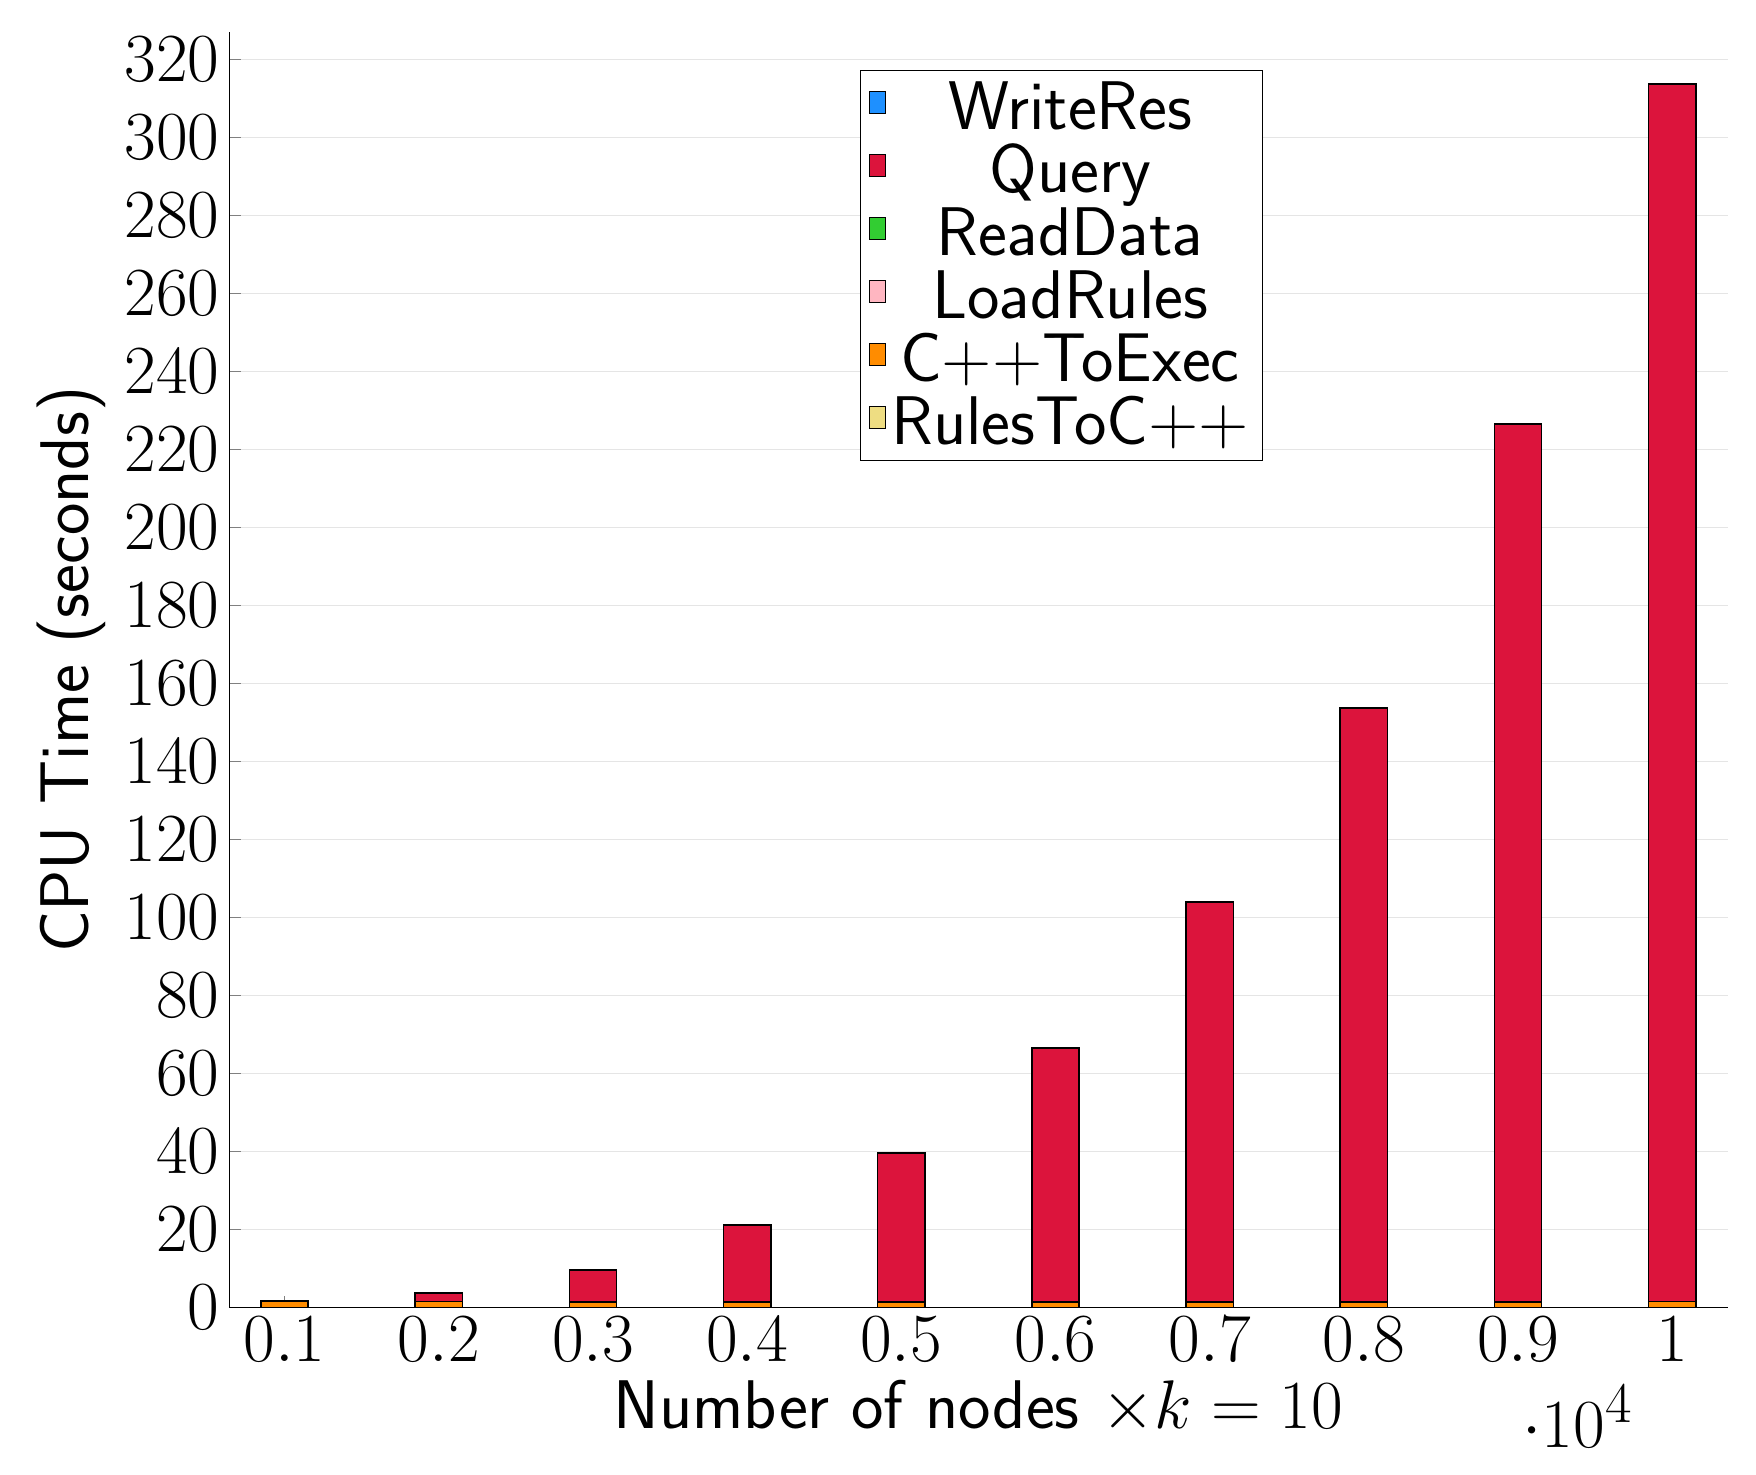
\begin{tikzpicture}
\begin{axis}[
   ybar stacked,
   width=1.7\textwidth,
   bar width=0.6cm,
   ymajorgrids, tick align=inside,
   major grid style={draw=gray!20},
   xtick=data,
   ymin=0, ymax=326.9108,
   axis x line*=bottom,
   axis y line*=left,
   enlarge x limits=0.04,
   legend style={
       at={(0.69, 0.97)},
       anchor=north east,
       legend columns=1,
       font=\Huge,
   },
   ylabel={CPU Time (seconds)},
   xlabel={Number of nodes $\times k=10$},
   label style={font=\Huge},
   tick label style={font=\Huge},
]
\addlegendimage{fill=DodgerBlue, draw=black, line width=0.2pt}
\addlegendentry{WriteRes}
\addlegendimage{fill=Crimson, draw=black, line width=0.2pt}
\addlegendentry{Query}
\addlegendimage{fill=LimeGreen, draw=black, line width=0.2pt}
\addlegendentry{ReadData}
\addlegendimage{fill=LightPink, draw=black, line width=0.2pt}
\addlegendentry{LoadRules}
\addlegendimage{fill=DarkOrange, draw=black, line width=0.2pt}
\addlegendentry{C++ToExec}
\addlegendimage{fill=LightGoldenrod, draw=black, line width=0.2pt}
\addlegendentry{RulesToC++}
\addplot +[fill=LightGoldenrod, draw=black, line width=0.55pt] coordinates {
(1000, 0.008000000000000002)
(2000, 0.004000000000000001)
(3000, 0.008000000000000002)
(4000, 0.011999999999999999)
(5000, 0.004000000000000001)
(6000, 0.006000000000000001)
(7000, 0.0020000000000000005)
(8000, 0.0)
(9000, 0.0020000000000000005)
(10000, 0.003999999999999997)
};
\addplot +[fill=DarkOrange, draw=black, line width=0.55pt] coordinates {
(1000, 1.482)
(2000, 1.486)
(3000, 1.4540000000000002)
(4000, 1.456)
(5000, 1.464)
(6000, 1.456)
(7000, 1.468)
(8000, 1.474)
(9000, 1.474)
(10000, 1.484)
};
\addplot +[fill=LightPink, draw=black, line width=0.55pt] coordinates {
(1000, 0.0001734)
(2000, 0.00018779999999999998)
(3000, 0.00019160000000000002)
(4000, 7.999999999999999e-05)
(5000, 0.0001558)
(6000, 0.00010040000000000001)
(7000, 0.0001712)
(8000, 0.0001494)
(9000, 0.0002134)
(10000, 0.00018839999999999997)
};
\addplot +[fill=LimeGreen, draw=black, line width=0.55pt] coordinates {
(1000, 0.0042642)
(2000, 0.005886)
(3000, 0.0087968)
(4000, 0.0080006)
(5000, 0.0143382)
(6000, 0.011474599999999998)
(7000, 0.018571200000000003)
(8000, 0.0201148)
(9000, 0.025695000000000003)
(10000, 0.029549799999999998)
};
\addplot +[fill=Crimson, draw=black, line width=0.55pt] coordinates {
(1000, 0.31416180000000005)
(2000, 2.208696)
(3000, 8.112143999999999)
(4000, 19.619419999999998)
(5000, 38.01953999999999)
(6000, 64.90376)
(7000, 102.46020000000001)
(8000, 152.1612)
(9000, 224.9568)
(10000, 311.9108)
};
\addplot +[fill=DodgerBlue, draw=black, line width=0.55pt] coordinates {
(1000, 0.002498)
(2000, 0.008849200000000002)
(3000, 0.019813000000000004)
(4000, 0.0349328)
(5000, 0.0540492)
(6000, 0.0775386)
(7000, 0.10575280000000001)
(8000, 0.13568960000000002)
(9000, 0.1721598)
(10000, 0.2114398)
};
\end{axis}
\end{tikzpicture}

\end{document}
